\setlength{\epigraphwidth}{.57\textwidth}
\begin{epigraphs}
\qitem{\textit{Statistics: the mathematical theory of ignorance.}}%
 {---\textsc{Morris Kline}}
\end{epigraphs}
Cosmology is intrinsically entwined with statistics. There are threefold reasons for this. Firstly, given the huge size of cosmological structure it is impossible to follow the evolution of all components in a deterministic way. Secondly, we do not observe  along a single spatial hyper-surface, rather we have direct observational access to our past light-cone, which means that we see objects at different stages of their evolution. Thirdly the generation of primordial inhomogeneities is an intrinsic stochastic process and as such, we can just predict the statistical properties of cosmological fields (such as the matter density contrast $\delta$ or the intensity of \gls{CMB} temperature fluctuations). The main implication of these remarks is that we should model the observable Universe as a stochastic \emph{realization} of a stochastic \emph{ensemble}. Moreover, in the vanilla inflationary framework, the initial perturbations are Gaussian and adiabatic meaning that the study of \gls{GRF}, with a specific focus on isotropic and homogeneous ones, is pivotal in cosmology. 

This chapter mainly deals with the methodology at the core of the analyses presented in this thesis and with the exploited datasets. We start by describing cosmological random fields with a special focus on the mathematics on the sphere. Then, we discuss the spectral estimation problem in the light of cosmological surveys, while in the last part of the chapter we present the \textit{Planck} and \textit{Herschel} datasets. 


\section{Random Fields}
\label{sec:RF}

\subsection{3D Random Fields}
We can describe a perturbation (calculated at a given time $t$) as a random field $f(\bm{x})$, which basically means that we assign a random number at each point $\bm{x} \in \mathbb{R}$ according to a probability density function $\text{P}[f(\bm{x})]$.\footnote{We will consider \emph{centered} field, i.e. $\langle f(\bm{x})\rangle=0$ for the sake of clarity. This is not an issue since the mean can always be subtracted from the field.} Here, $\text{P}[f(\bm{x})]$ is a distribution that gives the probability of realizing a particular field configuration.\footnote{The probability that the field $f$ will have a given configuration between $f(\bm{x})$ and $f(\bm{x})+\diff f(\bm{x})$ is calculated as $\diff P=\text{P}[f(\bm{x})]\Pi_{\bm{x}}\diff f(\bm{x})\equiv \text{P}[f(\bm{x})]\mathcal{D}f$.} Strictly speaking, a random field is a collection of $N$ random variables $f(\bm{x}_i)$ with $x_i \in \mathbb{R}^n$; the set of functions is called an \emph{ensemble} while each individual function represents a \emph{realization} of the ensemble. 

The correlators of the fields are the expectation values of the product of the field at different locations (and times). The \gls{2PCF} is defined~by
%
\be
\label{eq:RF_2point}
\xi(\bm{x},\bm{y}) \equiv \langle f(\bm{x})f(\bm{y})\rangle = \int \mathcal{D}f\, \text{P}[f]f(\bm{x})f(\bm{y}),
\ee
%
where the integral is a functional integral (or path integral) over the field configurations. The requirements of statistical isotropy and homogeneity translate into the following constraints on the correlation function: $\xi(\bm{x},\bm{y})=\xi(R^{-1}\bm{x},R^{-1}\bm{y})$ for the former and $\xi(\bm{x},\bm{y})=\xi(\bm{x}-\bm{y})$ for the latter, where $R$ is a generic rotation matrix. Combining the two together we find that the \gls{2PCF} only depends on the distance between points, i.e. $\xi(\bm{x},\bm{y}) = \xi(|\bm{x}-\bm{y}|)$. The same calculations can be performed in the harmonic domain by Fourier transforming the field adopting the following convention:
%
\be
f(\bm{k}) = \int \diff^3x\, f(\bm{x})e^{-i\bm{k}\cdot\bm{x}} \quad \text{and} \quad f(\bm{x}) = \int \frac{\diff^3k}{(2\pi)^{3}}f(\bm{k})e^{i\bm{k}\cdot\bm{x}}
\ee
%
Generically the Fourier transform is complex but for real valued fields we have that $f(\bm{k}) = f^*(-\bm{k})$. Then, the \gls{2PCF} in Fourier space than reads as
%
\be
\begin{split}
\langle f(\bm{k})f^*(\bm{k'}) \rangle &= (2\pi)^3 \delta^D(\bm{k}-\bm{k'}) \frac{2\pi^2}{k^3}\mathcal{P}_f(k)\\
&= (2\pi)^3 \delta^D(\bm{k}-\bm{k'}) P_f(k)
\end{split}
\ee
%
where $\mathcal{P}_f(k)$ is the \emph{dimensionless power spectrum} and the homogeneity and isotropy are enforced by the delta function and the dependence only on the module of $k$. The \gls{2PCF} and the power spectrum are a Fourier transform pairs:
%
\be
\label{eq:RF_xipk}
\begin{split}
\xi(\bm{x},\bm{y}) = \langle f(\bm{x})f(\bm{y})\rangle &= \int \frac{\diff^3 k}{(2\pi)^{3}}\frac{\diff^3 k'}{(2\pi)^{3}} \langle f(\bm{k})f^*(\bm{k'})\rangle e^{i\bm{k}\cdot\bm{x}}e^{i\bm{k'}\cdot\bm{y}} \\
&= \frac{1}{4\pi}\int \diff\log{k}\, \mathcal{P}_f(k)\int \diff \Omega e^{i\bm{k}\cdot(\bm{x}-\bm{y})}.
\end{split}
\ee
%
After the angular integration, Eq.~\eqref{eq:RF_xipk} reduces to
%
\be
\xi(\bm{x},\bm{y}) = \int \diff\log{k} \mathcal{P}_f(k) j_0(k|\bm{x}-\bm{y}|),
\ee
%
where $j_0(x) = \sin{x}/x$ and the variance is computed as the \gls{2PCF} at zero-lag,
%
\be
\sigma^2 = \xi(0) = \int \diff\log{k}\, \mathcal{P}_f(k).
\ee
%
Higher-order correlations can be evaluated by averaging the product of $n$ fields; some of the most studied polyspectra are the 3PCF or \emph{bispectrum}
%
\be
\langle f(\bm{k}_1)f(\bm{k}_2)f(\bm{k}_3)\rangle = (2\pi)^3 B(\bm{k}_1,\bm{k}_2,\bm{k}_3)\delta^D(\bm{k}_1+\bm{k}_2+\bm{k}_3),
\ee
%
and the 4PCF or \emph{trispectrum}
%
\be
\langle f(\bm{k}_1)f(\bm{k}_2)f(\bm{k}_3)f(\bm{k}_4)\rangle = (2\pi)^3 T(\bm{k}_1,\bm{k}_2,\bm{k}_3\bm{k}_4)\delta^D(\bm{k}_1+\bm{k}_2+\bm{k}_3+\bm{k}_4).
\ee
%

\myparagraph{Gaussian Random Field}
This class of random fields is of particular relevance in cosmology due to the high-level of Gaussianity predicted by inflation for primordial fluctuations. For (homogeneous and isotropic) \gls{GRF}, $\text{P}[f(\bm{x})]$ is a Gaussian functional of $f$ fully characterized by its power spectrum\footnote{Since the mean is zero.}, or by the \gls{2PCF} equivalently. If we discretize the field in $N$ pixels and represent it  as a collection of $f_i=f(\bm{x}_i)$ in a $N$-dimensional vector $\bm{f}=[f_1,f_2,\dots,f_N]^T$, the multivariate joint probability distribution of the \gls{GRF}  has the following form
%
\be
\text{P}[\bm{f}] \propto \frac{e^{-f_i \text{C}^{-1}_{ij}f_j}}{\sqrt{\text{det}(\text{C})}},
\ee
%
where C$_{ij}=\langle f_i f_j\rangle$ is the covariance matrix. Since the Gaussian is even under parity around the mean, any odd expectation value vanishes, e.g. $\langle f(\bm{x_1})f(\bm{x_2})f(\bm{x_3})\rangle = 0$, while any even higher-order correlation function can be written as sum of \gls{2PCF} products: this result is known as \emph{Wick's theorem} (or Isserlis theorem) and can be expressed as 
%
\be
\langle f(\bm{x_1})f(\bm{x_2})f(\bm{x_3})f(\bm{x_4})\dots\rangle = \sum \text{All possibile 2-point contractions}.
\ee
%

\subsection{Fields on the sphere}
\label{sec:harmanalysis}
Nearly all cosmological observations, from CMB to galaxy surveys, provide us with a sampling of 3D random fields projected on the sphere, mostly in the form of two-dimensional sky-maps.\footnote{This especially applies when distance information about the sources is unavailable, nevertheless the quantity of interest can always be projected on the sphere, as is the case for tomographic analyses of \gls{LSS}.}
The information content hidden in such maps is usually probed by means of harmonic analysis on the sphere. A popular observable that characterizes the statistical properties of a given cosmic field is the
angular power spectrum $C_{\ell}$ and its reconstruction enables a direct comparison between
models and data.

It is common practice to decompose the observed field $X(\nver)$ into spherical harmonics, a frequency-space orthonormal basis for square-integrable, i.e. $\int_{\mathbb{S}^2}\diff \Omega |X(\nver)|^2 < \infty$, as:
%
\begin{equation}
X(\nver) = \sum_{\ell=0}^{\infty} \sum_{m=-\ell}^{\ell} x_{\ell m}Y_{\ell m}(\nver),
\label{eqn:spharm}
\end{equation}
%
where the spherical harmonic coefficients are given by
%
\begin{equation}
\label{eqn:sphcoeff}
x_{\ell m} = \int_{\mathbb{S}^2}X(\nver)Y^*_{\ell m}(\nver)d\Omega.
\end{equation}
%
The spherical harmonics $Y_{\ell m}$ are the eigenfunctions of the Laplacian on the sphere $\nabla^2_{\mathbb{S}^2}=\frac{1}{\sin\theta}\frac
{\partial}{\partial\theta}
\left(\sin\theta\frac{\partial}{\partial\theta}\right)+\frac{1}{\sin^2\theta}\frac{\partial^2}{\partial\varphi^2}$, and are described by two integers, the \emph{multipole} $\ell$ and the azimuthal parameter $m$ that satisfy $\nabla^2_{\mathbb{S}^2} Y_{\ell m} = -\ell(\ell+1)Y_{\ell m}$ and $\partial_{\varphi} Y_{\ell m}= imY_{\ell m}$. We recall below some useful properties:
%
\begin{align}
\int_{\mathbb{S}^2} \diff\Omega\, Y_{\ell m}(\nver)Y^*_{\ell' m'}(\nver) &= \delta^K_{\ell\ell'}\delta^K_{mm'} &\text{Orthonormality}\\
\sum_{\ell m} Y_{\ell m}(\nver)Y^*_{\ell m}(\nver') &= \delta^D(\nver-\nver') &\text{Completeness} \\
\sum_m Y_{\ell m}(\nver)Y^*_{\ell m}(\nver') &= \frac{2\ell+1}{4\pi} P_{\ell}(\nver\cdot\nver') &\text{Addition Theorem} 
\end{align}
%
where $P_{\ell}(x)$ are the usual Legendre polynomials. The phase of $Y_{\ell m}$ can be chosen such  that $Y^*_{\ell m} = (-1)^mY_{\ell\, -m}$, so that for a real valued field we have $x^*_{\ell m}=(-1)^m x_{\ell\,-m}$.

Under the assumption of statistical isotropy, for a finite variance field, the mean of the spherical harmonic coefficients is $\langle x_{\ell m}\rangle = 0$, while their covariance is given by 
%
\be
\langle x_{\ell m} x^*_{\ell' m'}\rangle = C^{XX}_{\ell}\delta^K_{\ell\ell'}\delta^K_{mm'},
\ee
%
where $C_{\ell}^{XX}$ is the \emph{angular power spectrum} of $X$ which is related to the angular \gls{2PCF} $C^{XX}(\theta)$ through (see Eq.~\eqref{eq:c2cl} for the derivation)
%
\begin{align}
C^{XX}(\theta) &= \sum_{\ell}\frac{2\ell+1}{4\pi}C_{\ell}^{TT}P_{\ell}(\nver\cdot\nver')\\
C_{\ell}^{XX} &= 2\pi\int_{-1}^{1} \diff\cos{\theta}\, C^{XX}(\theta)P_{\ell}(\cos{\theta}).
\end{align}
%
It is also possible to expand the product of two spherical harmonics in terms of spherical harmonics as 
%
\be
Y_{\ell m}(\nver)Y_{\ell'm'}(\nver) = \sum_{LM} \sqrt{\frac{(2\ell+1)(2\ell'+1)(2L+1)}{4\pi}} \wig{\ell}{\ell'}{L}{m}{m'}{M}\wig{\ell}{\ell'}{L}{0}{0}{0} Y_{LM}^*(\nver),
\ee
%
where the strange quantities in parenthesis that we have introduced are called the Wigner $3j$ symbols \citep{Varshalovich1988}. Integrating the above expression over the whole sphere one finds the \emph{Gaunt relation}:
%
\be
\begin{split}
\mathcal{G}^{\ell\ell'L}_{mm'M} &\equiv \int_{\mathbb{S}^2}\diff\Omega\,Y_{\ell m}(\nver)Y_{\ell'm'}(\nver)Y_{LM}(\nver)\\
&= \sqrt{\frac{(2\ell+1)(2\ell'+1)(2L+1)}{4\pi}} \wig{\ell}{\ell'}{L}{0}{0}{0}\wig{\ell}{\ell'}{L}{m}{m'}{M}.
\end{split}
\ee
%
Basically, Wigner $3j$ matrices are a rescaling of the Clebsch-Gordan coefficients and describe the quantum mechanical composition of two angular momentum eigenstates into a third one.
The selection rules for Wigner $3j$ symbols, i.e. when they are non-null, are given by
%
\begin{align}
\ell + \ell' + L & \,\,\text{is even,} \\
|\ell-\ell'| \le L &\le \ell+\ell' \\
m + m' + M& = 0.
\end{align}
%
These objects are somewhat nasty to calculate and are at the core of the \gls{PCL} methods to calculate the masking induced mode-coupling, as we will see in Sec.~\eqref{sec:ps_est}. Harmonic calculations on the sphere can be performed on the computer with standard packages for \gls{CMB} data analysis such as \texttt{HEALPix}\footnote{\url{http://healpix.sourceforge.net}} \citep{Gorski2005a} and \texttt{S}$^2$\texttt{HAT} \citep{Stompor2011}. The basic idea is to tesselate the sphere according to some pixelization scheme and to discretize the function into maps. As an example, for \texttt{HEALPix}, the resolution of the grid is controlled by the parameter $N_{\rm{side}}=2^k$ (where $k \in \mathbb{N}$) which fixes the total number of pixels $N_{\rm{pix}}=12N_{\rm{side}}^2$. In particular, spherical harmonic transforms in Eq.~\eqref{eqn:sphcoeff} are operatively estimated as 
%
\be
x_{\ell m} \approx \Omega_p \sum_p X(p)Y^*_{\ell m}(p),
\ee
%
where $\Omega_p = \frac{4\pi}{N_{\rm{pix}}}$ is the solid angle subtended by each pixel $p$. Another complication that arises from pixelization is that we only know the value of the field averaged over the pixel area: the effect is an amount of degradation of the information below a certain scale set by the size of the pixel (basically it acts as a low-pass filter). A way to account for this bias is to deconvolve the reconstructed spectrum for the \emph{pixel window function} $p_{\ell}$ ($C_{\ell}^{\rm{obs}} = p^2_{\ell}C_{\ell}$).

Before concluding this subsection, let us take a look at the near future: most of the upcoming cosmological surveys will carry out large and deep observations of the sky, providing both angular and redshift information about the cosmic fields. Thus, a formalism  
for analyzing function on the 3D \emph{ball} -  a family of concentric spheres (shells) indexed by a continuos radial parameter, such as the redshift $z$ - will be required. Tomographical analyses (see Ch.~\eqref{ch:xc2}) represent a first step in this direction: the idea is to slice the data in redshift bins and then perform the usual 2D spherical analysis. A natural decomposition scheme for full-3D analyses is given by the spherical Fourier-Bessel formalism, while extensions to wavelets \citep{Lanusse2012,Leistedt2012} and radial 3D needlets \citep{Durastanti2014} have also been investigated.

\subsection{Projected fields}
Let us now work out the connection between a 3D field $X^{\rm 3D}(\bm{x})$ and its 2D counterpart $X^{\rm 2D}(\nver)$, projected
on the sphere and integrated along the light-cone according to some arbitrary weight function $W^X(\chi)$:\footnote{To avoid a crowding of equations we restrict to the case of a flat Universe, so that $f_K(\chi)=\chi$.}
%
\begin{equation}
X^{\rm 2D}(\nver) = \int_0^{\infty} \diff\chi\,  W^X(\chi) X^{\rm 3D}(\chi\nver,\chi).
\end{equation}
%
Using the Rayleigh's expansion
\begin{equation}
e^{i\mathbf{k}\cdot\nver\chi(z)} = 4\pi\sum_{\ell m}i^{\ell}j_{\ell}(k\chi)Y^*_{\ell m}(\kver)Y_{\ell m}(\nver),
\end{equation}
we can Fourier transform the 3D field $X^{\rm 3D}(\chi\nver,\chi)$ and obtain
%
\begin{equation}
\begin{split}
X^{\rm 3D}(\chi\nver, \chi) &= \int \frac{\diff^3k}{(2\pi)^3}\,X^{\rm 3D}(\mathbf{k}, \chi) e^{i\mathbf{k}\cdot\nver\chi} \\
&=4\pi\sum_{\ell m}i^{\ell}\int \frac{\diff^3k}{(2\pi)^3}\,X^{\rm 3D}(\mathbf{k}, \chi) j_{\ell}(k\chi)Y^*_{\ell m}(\kver)Y_{\ell m}(\nver).
\end{split}
\end{equation}
%
In this way, the projected field becomes
%
\begin{equation}
X^{\rm 2D}(\nver)= 4\pi\sum_{\ell m}i^{\ell}\int \diff\chi W^X(\chi) \int \frac{\diff^3k}{(2\pi)^3}X^{\rm 3D}(\mathbf{k}, \chi) j_{\ell}(k\chi)Y^*_{\ell m}(\kver)Y_{\ell m}(\nver),
\end{equation}
%
and the spherical coefficients read as 
\begin{equation}
x_{\ell m} =4\pi i^{\ell} \int \diff\chi\, W^X(\chi) \int \frac{\diff^3k}{(2\pi)^3}\,X^{\rm 3D}(\mathbf{k}, \chi) j_{\ell}(k\chi)Y^*_{\ell m}(\kver).
\end{equation}
We calculate the angular cross power spectrum $C_{\ell}^{XY}$ by taking the ensemble average of $\langle x_{\ell m}y^*_{\ell m}\rangle $ as 
%
\begin{equation}
\begin{split}
C_{\ell}^{XY} =\:&  (4\pi)^2 \int \diff\chi\, W^X(\chi)\int \diff\chi'\, W^X(\chi')\\
&\times \int\frac{\diff^3k}{(2\pi)^3}\frac{\diff^3k'}{(2\pi)^3}\langle X^{\rm 3D}(\mathbf{k}, \chi) Y^{\rm 3D*}(\mathbf{k'}, \chi') \rangle 
 j_{\ell}(k\chi)j_{\ell'}(k'\chi')Y^*_{\ell m}(\kver)Y_{\ell' m'}(\kver') \\
=\:& (4\pi)^2 \int \diff\chi\, W^X(\chi)\int \diff\chi'\, W^Y(\chi')\int\frac{\diff^3k}{(2\pi)^3}  P_{XY}(k;\chi,\chi') j_{\ell}(k\chi)j_{\ell'}(k\chi')Y^*_{\ell m}(\kver)Y_{\ell' m'}(\kver) \\
=\:& \frac{2}{\pi}\int \diff\chi\, W^X(\chi)\int \diff\chi'\, W^Y(\chi')\int k^2\diff k\,  P_{XY}(k;\chi,\chi') j_{\ell}(k\chi)j_{\ell}(k\chi') 
\end{split}
\end{equation}
%
where we used the definition of (isotropic) 3D cross-power spectrum $\langle X(\mathbf{k}, \chi) Y^*(\mathbf{k'}, \chi')\rangle= (2\pi)^3\delta^D(\kvec-\kvec')P_{XY}(k;\chi,\chi')$ and the orthonormality condition of spherical harmonics. Summing up, the \emph{exact} relation is
%
\begin{equation}
\label{eq:clexact}
C_{\ell}^{XY} = \frac{2}{\pi}\int \diff\chi\, W^X(\chi)\int \diff\chi'\, W^Y(\chi')\int k^2\diff k\,  P_{XY}(k;\chi,\chi') j_{\ell}(k\chi)j_{\ell}(k\chi').
\end{equation}
% 
\myparagraph{Limber approximation}
The Limber approximation \citep{Limber1953a} is a handy tool whenever integrals of Bessel functions appear.
When deriving it, one usually assumes small angular separations (or large multipoles $\ell$) and that some of the integrand functions vary slower with respect to others. The idea is that if $f(x)$ is a smooth function, then $\int_0^{\infty} \diff x f(x)J_{\nu}(x) = f(\nu) + \mathcal{O}(1/\nu^2)$, where $\nu \equiv \ell + 1/2$; this can be written in the following form
%
\begin{equation}
\frac{2}{\pi}\int k^2\diff k\, f(k) j_{\ell}(k\chi)j_{\ell}(k\chi') = \frac{\delta^D(\chi-\chi')}{\chi^2} f\biggl(\frac{\nu}{\chi}\biggr)\biggl[1+\mathcal{O}\biggl(\frac{1}{\nu^2}\biggr)\biggr],
\end{equation}
%
where the presence of the $\delta^D$ tells us that the integrand is dominated by the region $\chi \approx \chi'$, and the goodness of the approximation gets better as $\ell\to\infty$, i.e. the corrections are $\mathcal{O}(1/\nu^2)$ (see \citet{LoVerde2007}).
Substituting the above expression in Eq.~\eqref{eq:clexact} (and integrating out the $\delta^D$), one finds the Limber approximated angular power spectrum:
%
\be
\label{eq:cllimber}
C_{\ell}^{XY} = \int_0^{\infty} \frac{\diff\chi}{\chi^2}W^X(\chi)W^Y(\chi) P_{XY}\Biggl(\frac{\ell+\frac{1}{2}}{\chi},\chi\Biggr). 
\ee
%
In literature the power spectrum in Eq.~\eqref{eq:cllimber} is sometimes evaluated at $\nu = \ell$ (as will be the case in Ch.~\eqref{ch:xc1} and \eqref{ch:xc2}), which increase the error from $\mathcal{O}(\ell^{-2})$ to $\mathcal{O}(\ell^{-1})$. The approximation is correct to $\mathcal{O}(1\%)$ for $\ell \gtrsim 10$. An extended Limber approximation, in the sense that exploits higher-order terms in the Bessel integral expansion, has been developed by \citet{LoVerde2007}. For completeness, we write below the analogous of Eq.~\eqref{eq:cllimber} with the integration in redshift space:\footnote{In order to switch the Dirac delta from $\chi$ to $z$ recall that $\delta^D[g(x)]=\frac{\delta^D(x-x_0)}{|g'(x_0)|}$ where $x_0$ is the root of $g(x)$. In our case $g(z)=\chi(z)-\chi(z')=\int_0^z\frac{c\,dz''}{H(z'')}-\int_0^{z'}\frac{c\,dz''}{H(z'')}$, so that $g'(z)=\frac{c}{H(z)}$ and $\delta^D[\chi(z)-\chi(z')] = \frac{H}{c}(z')\delta^D(z-z')$}
\be
\label{eq:cllimber_z}
C_{\ell}^{XY} = \int_0^{\infty} \frac{\diff z}{c} \frac{H(z)}{\chi^2(z)}W^X(z)W^Y(z) P_{XY}\Biggl(\frac{\ell+\frac{1}{2}}{\chi(z)},z\Biggr). 
\ee
Recall that the comoving distances $\chi$ should be replaced by $f_K(\chi)$ for non-flat cosmologies and that Limber approximation is valid as long as (i) the sources stretch in a \emph{wide} range of distances $\Delta\chi$ and (ii) vary smoothly, i.e. $\ell/\chi\times\Delta\chi \gg 1$ (see \citet{Simon2007,Bernardeau2011}).

\section{Spectral estimation}
\label{sec:ps_est}
The scientific exploitation of any cosmological dataset is just the tip of the iceberg: the data analysis that allows us to extract science from observations is a complex and iterative process which requires both computational and physical solid skills. Having in mind the \gls{CMB} field, the reduction of a dataset usually can be split in the following sequence of steps:
\begin{itemize}
\item{\textbf{Pre-processing}: the goal is to prepare real data so that can be fed to the subsequent pipeline steps. Here, the raw time-ordered data (TOD) collected by the detectors are calibrated and the time-domain systematics are generally flagged and/or removed.}
\item{\textbf{Map-making}: after characterizing the instrument's noise specifics, the different frequency maps of the observed temperature and polarization are extracted from the cleaned TOD.}
\item{\textbf{Component separation}: the available spectral information is used to isolate the emission from all other (astrophysical) components in the data, hence singling out the \gls{CMB} signal. One of the outcome of this pipeline step is the production of ancillary data. Though not strictly correct, we can insert in this step the production of additional maps, such as the \gls{CMB} gravitational lensing convergence, derived from the $T$ and $P$ separated maps.}
\item{\textbf{Power spectrum estimation}: \gls{CMB} temperature $T$ and polarization $E$- and $B$- modes auto- and cross-power spectra are reconstructed from the maps, along with spectra of derived fields such as lensing $\kappa$.}
\item{\textbf{Parameter estimation}: the estimated set of \gls{CMB} power spectra is compared with the theoretical models to study the degeneracies in the parameter space and infer best-fit parameters, usually by means of Bayesian analysis.}
\end{itemize}

\subsection{Power spectrum estimators}
\label{sec:ps_est_master}
Throughout  my thesis I have mainly been involved with the last two steps of the \gls{CMB} pipeline, here I will focus on the power-spectrum estimation techniques: since the statistical properties of \gls{GRF} are completely described by their power spectra, spectral estimation is a pivotal step.

There exist a variety of well-established methods to recover the underlying angular spectra from observations. In principle, optimal maximum likelihood algorithms can be applied to the spectral estimation problem, assuming that the pixel-pixel covariance matrix is known. The idea behind these methods is the following: considering a data vector $x_i$ (e.g. the \gls{CMB} temperature in a given pixel) of length $N_d$ with the $x_i$ being Gaussian distributed, then the likelihood function reads as
%
\be
\mathcal{L}(C_{\ell}|\bm{x}) = \frac{\exp{\bigl(-\frac{1}{2}x^T C^{-1} x\bigr)}} {\sqrt{(2\pi)^{N_d} \text{det}(C)}}.
\ee
%
Here $C_{\ell}$ is the power spectrum to be estimated and the covariance matrix $C$ (in pixel space) can be written as the sum of signal $S_{ij}$ and noise $N_{ij}$ terms as $C_{ij}=\langle x_ix_j\rangle=S_{ij}(C_{\ell})+N_{ij}$. From this, maximum likelihood solution can be found iteratively with Newton-Raphson algorithm \citep{Bond1998} or with quadratic maximum likelihood estimators \citep{Tegmark1997}. Despite being optimal, these methods are computational expensive and require $\mathcal{O}(N_{\rm{pix}}^3)$ CPU time (as well as a good knowledge of the covariance matrix), and become prohibitively for datasets with $N_{\rm{pix}} \gtrsim 10^5$. 

As a result, \gls{PCL} techniques have emerged on the market, see \citet{Yu1969,Hauser1973,Wandelt2001,Hivon2001a,Efstathiou2004a}. The idea is to split the estimation of $C_{\ell}$ in two steps: a biased estimate $\tilde{C}_{\ell}$ of the power spectrum is first obtained, and then  corrected in the harmonic domain for all the different biasing effects such as the beam function, the pixelization, the mapmaking, and mode-mode coupling induced by masking. Schematically, the true power spectrum and the initial estimate are related by the mapping $\tilde{C_{\ell}}= f(C_{\ell})$, where the function $f$ encodes all the biasing effects. If we linearly expand it, we can rewrite the previous relation in matrix notation as $\langle\tilde{C}_{\ell'}\rangle \approx \sum_\ell \alpha_{\ell'\ell}C_{\ell} + \beta_{\ell'}$, where $\{\alpha_{\ell'\ell}, \beta_{\ell'}\}$ are the coefficients that approximate the effect of $f$, and then invert it to recover the true spectrum as $\hat{C}_{\ell'} = \alpha^{-1}_{\ell'\ell}(\tilde{C}_{\ell}-\beta_{\ell})$. 
The \gls{PCL} method is very fast, requiring $\mathcal{O}(N_{\rm{pix}}^{3/2})$ CPU time and it is nearly-optimal for temperature (and scalar fields) in practice.\footnote{The problem with the estimation of polarized spectra is the spurious mixing of $E$- and $B$-modes ($E$-to-$B$ leakage) that has to be taken into account. Several methods have been proposed to treat such effect, see \citet{Lewis2001,Bunn2003,Grain2009}.} Let us see the details of the method (for spin-0 fields).

From a statistical point of view, an unbiased estimator of the (cross-)angular power spectrum is given by (hereafter the hat $\hat{X}$ 
denotes  estimated quantities):
%
\begin{equation}
\label{eq:cl_est}
\hat{C}_{\ell}^{XY} = \frac{1}{2\ell+1}\sum_{m=-\ell}^{\ell} x_{\ell m}y_{\ell m}^*.
\end{equation}
%
%$\hat{C}_{\ell}$ can be shown to possess the minimal variance among the unbiased 
%estimators (in the sense that its variance reaches the Cram\`er-Rao lower bound).
Spherical harmonics are particularly appealing because they are statistically orthogonal for full-sky 
Gaussian-distributed sky-maps, i.e. the covariance is diagonal $\text{Cov}_{\ell \ell'}\propto \delta^K_{\ell
\ell'}$, and the power spectrum fully characterizes the behavior of the field. However, real-world observations have to deal with
a number of limitations and issues, such as the finite instrumental spatial resolution, the anisotropic 
noise, and asymmetric beam response. Moreover the incomplete sky coverage, motivated for example 
by foreground contamination or the instruments scanning strategy, induces a mode-coupling and a power leakage between 
different multipoles, as well as an overall downward shift of power \citep{Hivon2001a,Efstathiou2004a}. 
Consider a position dependent weighting scheme $W(\nver)$, i.e. the mask, whose harmonic expansion is $W(\nver)=\sum_{\ell m} w_{\ell m}Y^*_{\ell m}(\nver)$ and its power spectrum is $\mathcal{W}_{\ell}$. Then the pseudo-$x_{\ell m}$ of the masked field $\tilde{X}(\nver)=X(\nver)W(\nver)$ are given by:
%
\begin{equation}
\begin{split}
\tilde{x}_{\ell m} &= \int_{\mathbb{S}^2}X(\nver)W(\nver)Y^*_{\ell m}(\nver)d\Omega \\
&= \sum_{\ell'm'} x_{\ell'm'} \int\diff\Omega \, Y_{\ell'm'}(\nver) W(\nver)Y^*_{\ell m}(\nver)\\
&= \sum_{\ell' m'} K_{\ell m \ell' m' }[W] x_{\ell' m'},
\end{split}
\label{eqn:sphcoeffmask}
\end{equation}
%
where the kernel $K$  that describes the induced mode-coupling reads as
%
\be
K_{\ell m \ell' m' }[W]  \equiv (-1)^m \sum_{\ell'' m''} w_{\ell'' m''} \gaunt{\ell}{\ell'}{\ell''}{m}{m'}{m''}.
\ee
%
The well known \texttt{MASTER} \citep{Hivon2001a} (or \texttt{XSPECT}, the cross-spectra extension by \citet{Tristram2005}) approach to obtain unbiased but slightly sub-optimal multipole estimates relates the pseudo-spectrum 
%
\be
\tilde{C}^{XY}_{\ell} = \frac{1}{2\ell+1} \sum_m \tilde{x}_{\ell m}\tilde{y}^*_{\ell m}
\ee
%
to the underlying power spectrum $C_{\ell}$ as 
%
\begin{equation}
\label{eqn:pcl2cl}
\langle \tilde{C}^{XY}_{\ell}\rangle = \sum_{\ell'} M_{\ell\ell'} C^{XY}_{\ell'},
\end{equation}
%
where $M_{\ell\ell'}$ is the \emph{coupling matrix} 
%
\be
M_{\ell\ell'} = \frac{2\ell'+1}{4\pi} \sum_{\ell''} (2\ell''+1) \mathcal{W}_{\ell''} \wig{\ell}{\ell'}{\ell''}{0}{0}{0}^2
\ee
%
The finite size of the observed sky patch (of area $A_{\rm{obs}}$) approximately determines the smaller multipole that can be recovered, 
$\ell_{\rm{min}}\approx \pi/\sqrt{A_{\rm{obs}}}$, and the width of $M_{\ell\ell'}$, that characterizes the amount of mode-coupling.  
The basic idea is to invert eq.~\eqref{eqn:pcl2cl} in order to 
recover the underlying power spectrum, however for small sky fraction  $f_{\rm{sky}}=\frac{1}{4\pi}\int_{\mathbb{S}^2}W^2(\nver)d\Omega$, 
one needs to bin the pseudo-power spectrum and the coupling matrix, so that the estimator of the true
 cross-bandpowers $\hat{C}^{XY}_{L}$ writes
%
\begin{equation}
\label{eqn:master_xy}
\hat{C}^{XY}_{L} = \sum_{L' \ell}K^{-1}_{LL'}P_{L'\ell}\tilde{C}^{XY}_{\ell},
\end{equation}
%
where $L$ is the bandpower index and the binned coupling matrix can be written as
%
\begin{equation}
K_{LL'} = \sum_{\ell\ell'} P_{L\ell}M_{\ell\ell'}B^X_{\ell'}B^Y_{\ell'}p^2_{\ell'}F_{\ell'}Q_{\ell' L'}.
\end{equation}
%
Here $P_{L\ell}$ is the binning operator and $Q_{\ell L}$ is its reciprocal. To correct also for angular resolution, finite pixel size and filtering applied to TOD, we added to the binned coupling matrix the beam function (for the observed field $X$) $B^X_{\ell'}$, the pixel window function $p_{\ell}$, and the effective filtering function $F_{\ell'}$. When dealing with auto-power spectra of maps comprehensive of noise, Eq.~\eqref{eqn:master_xy} gets modified as
%
\begin{equation}
\label{eqn:master_xx}
\hat{C}^{XX}_{L} = \sum_{L' \ell}K^{-1}_{LL'}P_{L'\ell}(\tilde{C}^{XX}_{\ell} - \langle \tilde{N}^{XX}_{\ell} \rangle_{\rm{MC}}),
\end{equation}
%
where $\langle \tilde{N}^{XX}_{\ell} \rangle_{\rm{MC}}$ is the \gls{MC} estimate of the average noise pseudo-power spectrum.
If the true power spectrum varies slowly with respect to the coupling matrix and/or $f_{\rm{sky}}$ is large, eq.~\eqref{eqn:pcl2cl} becomes  
%
\begin{equation}
\label{eqn:fsky_app}
\langle \tilde{C}^{XY}_{\ell}\rangle \approx  C^{XY}_{\ell}  \sum_{\ell'} M_{\ell\ell'} = f_{\rm{sky}} C^{XY}_{\ell},
\end{equation}
%
which is the so-called $f_{\rm{sky}}$ approximation \citep{Komatsu2002a}. For the analyses discussed in Ch~\eqref{ch:xc1} and \eqref{ch:xc2} and performed during my Ph.D., I have developed a code to compute coupling matrices and estimate power spectra of spin-0 masked maps. The computational bottleneck is represented by the calculation of the Wigner $3j$ symbols: to this end, I have wrapped the FORTRAN rc3jj.f routine from the \texttt{SLATEC} library\footnote{\url{http://www.netlib.org/slatec/}} into flexible Python code which calculates the coupling matrix $M_{\ell\ell'}$, as well as other quantities, and can be efficiently interfaced with usual \texttt{HEALPix}-based codes (such as the Python implementation called \texttt{healpy}\footnote{\url{https://healpy.readthedocs.io/en/latest/}}). Just as an illustration and example of how a coupling matrix can appear, we anticipate here the mapping in the case of the H-ATLAS dataset considered in this analysis.
In the left panel of Fig.~\eqref{fig:master} we show the \textit{unbinned} coupling matrix $M_{\ell\ell'}$ computed for the H-ATLAS mask (shown in the right panel of Fig.~\eqref{fig:masks}) that tells us how the different harmonic modes are coupled to each other. As previously mentioned, the width of the diagonal is roughly determined by the sky coverage and mask topology: to highlight this aspect, we plot slices through $M_{\ell\ell'}$ (at fixed $\ell'$) in the right panel of Fig.~\eqref{fig:master}.

\begin{figure} %1
\centering % \begin{center}/\end{center} takes some additional vertical space
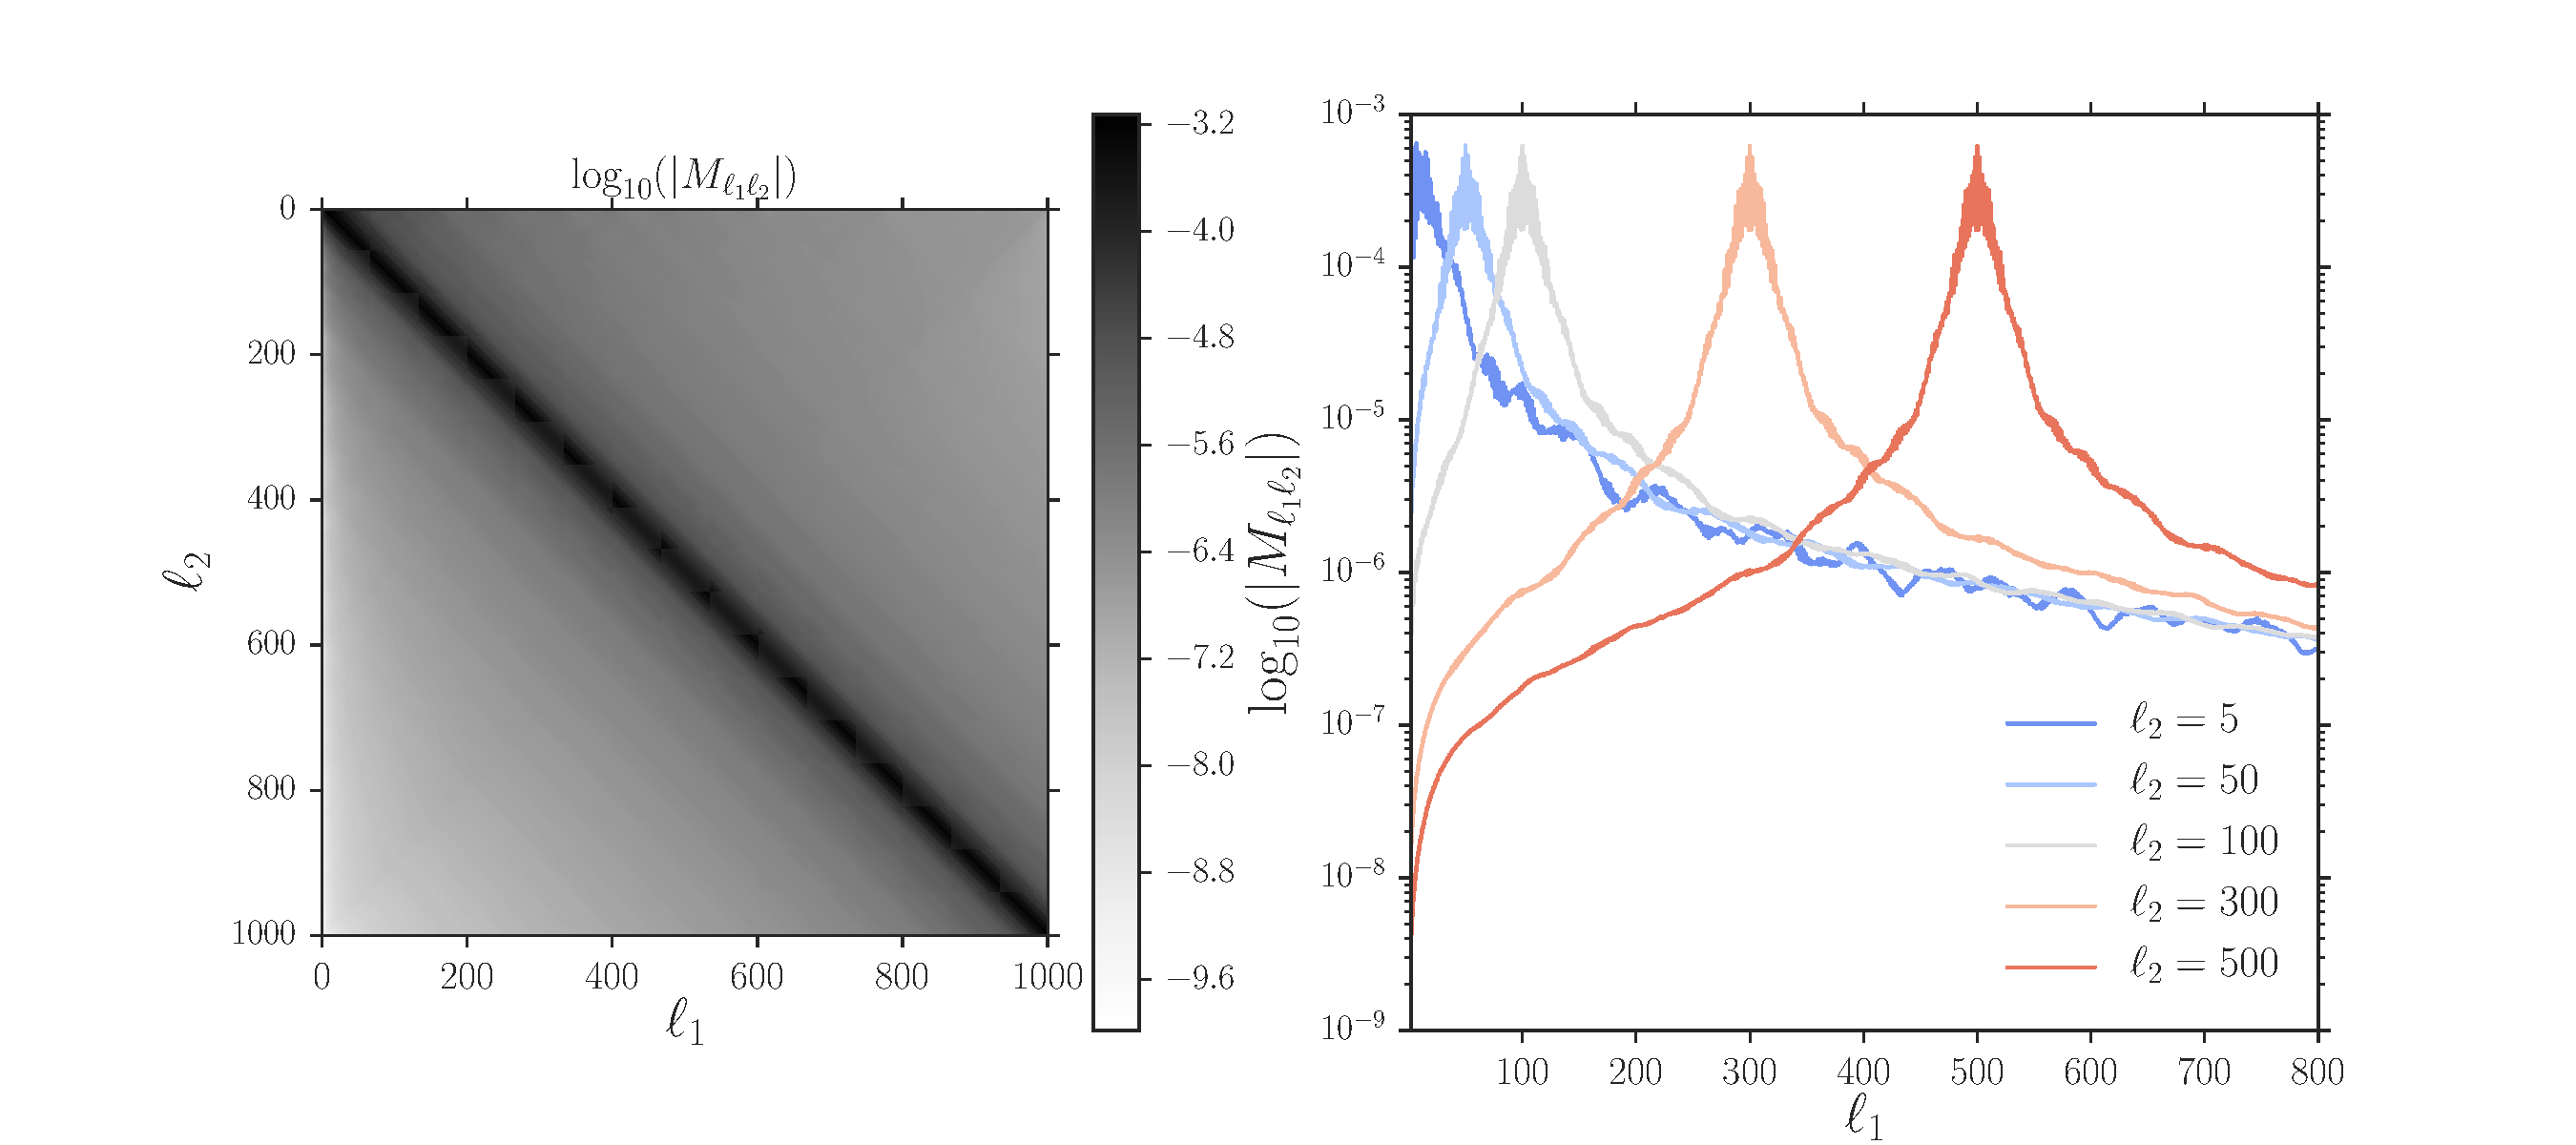
\includegraphics[width=\textwidth]{Chapter2/Images/master}
\caption{\emph{Left panel:} Coupling matrix $M_{\ell\ell'}$ evaluated for the H-ATLAS mask shown in Fig.~\eqref{fig:masks}. The main diagonal structure, whose width determines the extent of the mode-coupling, is visible. \emph{Right panel:} Slices through the coupling matrix shown in the left panel. \label{fig:master}}
\end{figure}

\subsection{Covariance estimators}
\label{sec:cov_est}
An estimate of the power spectrum means almost nothing without the associated covariance matrix. Error bars must be assigned to asses the quality or the significance of measurements and, for example, the full covariance matrix is needed to perform the further pipeline steps such as the parameter estimation. The covariance of the power spectrum estimator $\hat{C}_{\ell}^{XX}$ defined in Eq.~\eqref{eq:cl_est} is:\footnote{Assuming that the fields are Gaussian, hence neglecting the connected part $\langle  x_{\ell m}y^*_{\ell m}x_{\ell'm'}y^*_{\ell'm'}\rangle_c$.}
%
\be
\begin{split}
\cov(\hat{C}^{XY}_{\ell},\hat{C}^{XY}_{\ell'}) &= \langle (\hat{C}^{XY}_{\ell} - C^{XY}_{\ell}) (\hat{C}^{XY}_{\ell'} - C^{XY}_{\ell'}) \rangle \\
&= \frac{1}{(2\ell+1)(2\ell'+1)}\sum_{mm'} \langle x_{\ell m}y^*_{\ell m}x_{\ell'm'}y^*_{\ell'm'}\rangle - C^{XY}_{\ell}C^{XY}_{\ell'} -  \cancel{C^{XY}_{\ell}C^{XY}_{\ell'}}  \\
&\hphantom{=}+ \cancel{C^{XY}_{\ell}C^{XY}_{\ell'}}\\
&= \frac{1}{(2\ell+1)(2\ell'+1)}\sum_{mm'} \Bigl[\langle x_{\ell m}y^*_{\ell m} \rangle\langle x_{\ell' m'}y^*_{\ell' m'} \rangle  + \langle x_{\ell m}x_{\ell'm'} \rangle\langle y^*_{\ell m}y^*_{\ell' m'} \rangle \\
&\hphantom{=\frac{1}{(2\ell+1)(2\ell'+1)}\sum_{mm'} [}+ \langle x_{\ell m}y^*_{\ell' m'} \rangle\langle x^*_{\ell' m'}y^*_{\ell' m'} \rangle\Bigr] - C^{XY}_{\ell}C^{XY}_{\ell'}\\
&= \cancel{C^{XY}_{\ell}C^{XY}_{\ell'}} + \frac{C^{XX}_{\ell}C^{YY}_{\ell'}}{2\ell+1}\delta^K_{\ell\ell'} + \frac{C^{XY}_{\ell}C^{XY}_{\ell'}}{2\ell+1}\delta^K_{\ell\ell'} - \cancel{C^{XY}_{\ell}C^{XY}_{\ell'}} \\
&= \frac{\delta^K_{\ell\ell'}}{2\ell+1} \left[C^{XY}_{\ell}C^{XY}_{\ell'} + C^{XX}_{\ell}C^{YY}_{\ell'}\right]. 
\end{split}
\ee
%
Then, the cross- and auto-power spectrum variance associated to a given multipole are respectively
%
\begin{align}
\label{eq:thvar}
(\Delta C_{\ell}^{XY})^2 &= \frac{1}{2\ell+1}\left[(C^{XY}_{\ell})^2 + C^{XX}_{\ell}C^{YY}_{\ell}\right] \\
(\Delta C_{\ell}^{XX})^2 &= \frac{2}{2\ell+1}(C^{XX}_{\ell})^2,
\end{align}
%
with the last one being the same as Eq.~\eqref{eq:cmb_CV}. Let us make a couple of remarks. First of all, if the maps being analyzed are comprehensive of noise (as in the real-world), then the auto-power spectra appearing in the above equations must include a noise term, i.e. $C_{\ell}^{XX} \to C_{\ell}^{XX} + N_{\ell}^{XX}$. Secondly, in the incomplete sky case, things become much more nastier and a \emph{full} analytical treatment is virtually unfeasible. Several authors \citep{Efstathiou2004a,Tristram2005,Brown2005} have proposed analytic approximations if the underlying power spectra meet certain criteria, for example if they vary slow with respect to the coupling matrix. In the \emph{zeroth-order} approximate formula for power spectrum error bars, known as the Knox formula \citep{Knox1995}, the fractional error on $C_{\ell}$ typically scales as $1/\sqrt{f_{\rm{sky}}}$. Although it is helpful for an assessment of uncertainties, it is known to underestimate errors and does not account for the mode-mode coupling and the $E$-to-$B$ mixing. We will discuss in greater detail these approximations and compare different covariance estimators for cross-power spectra in Ch.~\eqref{ch:xc1}. The covariance can also be estimated numerically by means of MC simulations with resampling techniques. There exist different ways to calculate the covariance, each with their respective advantages and drawbacks. Here we list the most common  ones adopted in literature for cross-correlation analyses, mainly developed for \gls{iSW} studies, see \citet{Cabre2007,Giannantonio2008} for thorough discussions.

\begin{itemize}
\item{\textbf{\gls{MC} method 1}: Perhaps the most used estimator in literature, it consists in measuring the cross-power spectrum (or \gls{2PCF}) between $\Nsim$ random maps of field $X$, obtained from a fiducial model, and the observed maps of the field $Y$. This method is fast and straightforward to implement. \emph{Issues}: it is model-dependent (like all \gls{MC} approaches),  it does not account for the variance in the $Y$ maps (this is called the \emph{realization bias} since we have only one realization of the $Y$ field), and it assumes no cross-correlation between the fields (the so-called \emph{correlation bias}, but if the expected signal is weak, it should not represent a large bias).}
\item{\textbf{\gls{MC} method 2}: It tries to improve \gls{MC}1 by measuring the cross-power spectrum between random (\gls{MC} generated) maps of the $X$ field (from the underlying model) and random $Y$ field maps. \emph{Issues}: it is somewhat more time consuming and still model-dependent but has no dependence on any observed maps unlike the \gls{MC}1.}
\item{\textbf{Jack-knife (JK) method}: The idea is to divide the $Y$ field (e.g., the LSS tracer map) into $M$ patches to create $M$ subsamples (of approximately the same area) by neglecting each patch in turn and evaluating the covariance between them. \emph{Issues}: it underestimates the error, results are dependent on the size and number of discarded patches, it assumes independence of different patches (not always the case), but it is model-independent.}
\end{itemize}
The mock maps used to estimate covariances can either be obtained through \texttt{HEALPix} via the synfast routine, or from N-body simulations. But what are the errors on the errors? The number of simulations exploited is important in determining the covariance matrix estimation convergence: \citet{Taylor2013} have shown that the fractional noise in a covariance matrix of $N_d \times N_d$ elements, obtained from $\Nsim$ realizations, can be estimated as $\sqrt{2/(\Nsim - N_d - 4)}$.
To numerically estimate the covariance with \gls{MC}1 and \gls{MC}2 methods, one resorts to the sample covariance matrix:
%
\begin{equation}
\cov^{XY}_{LL'} = \frac{1}{\Nsim-1} \sum_{i=1}^{\Nsim} ( \hat{C}^{XY,i}_{L} - \langle \hat{C}^{XY}_{L}\rangle_{\rm MC})( \hat{C}^{XY,i}_{L'} - \langle \hat{C}^{XY}_{L'}\rangle_{\rm MC}),
\end{equation}
%
while for the JK method the estimator becomes
%
\begin{equation}
\cov^{XY}_{LL'} = \frac{M-1}{M} \sum_{i=1}^{M} ( \hat{C}^{XY,i}_{L} - \langle \hat{C}^{XY}_{L}\rangle)( \hat{C}^{XY,i}_{L'} - \langle \hat{C}^{XY}_{L'}\rangle).
\end{equation}
%

\section{Datasets}
As anticipated at the beginning of this Chapter, we dedicate the remaining part to provide a brief and introductory description of the most important datasets that we exploit in this thesis. The data, and their combination, will be treated and discussed quantitatively in the following chapters. 

\label{sec:datasets}
\subsection{Planck}
The \textit{Planck} satellite is a European Space Agency (ESA) mission devised to the measurement of \gls{CMB} anisotropies and it represents the third generation of spatial missions devoted to \gls{CMB} physics, after COBE and WMAP. It was launched on 14th May 2009 (together with its companion ESA's \textit{Herschel} satellite) towards the second Lagrangian point L2 and has collected data until October 2013. The \emph{nominal mission} data, released in 2013, consists in 15 months of temperature-only observations, while the \emph{full mission} data comprehends all the 30 months of the High Frequency Instrument  (see below) temperature and polarization data. 

The \textit{Planck} telescope is an off-axis tilted Gregorian design, with the optical system composed by a primary mirror of about 1.5 m and the secondary, which focuses the radiation to the detectors, of about 1 m. Their operative temperature is approximately 45 K. \textit{Planck}'s focal plane contains two separate scientific instruments: the Low Frequency Instrument (LFI) \citep{Bersanelli2010}, an array of radiometers covering three bands centered in 30, 44, and 70 GHz, and the High Frequency Instrument (HFI) \citep{Lamarre2010}, and array of microwave spider-web bolometers operating at higher frequencies from 100 GHz to 857 GHz. Corrugated horns serve as wave-guides to collect the radiation to the instruments detectors. Below we provide a brief description of the two intstruments:
%
\begin{itemize}
\item{\textbf{HFI}: it observes the sky in six frequency bands centered at 100, 143, 217, 353, 545, and 857 GHz, thus allowing for a characterization of the cosmological \gls{CMB} signal and to study both Galactic and extragalactic foregrounds. HFI detectors are bolometers that, depending on the placement on the grid wires, can be sensitive only to the intensity of the incoming radiation or to polarization as well. The former are called spider-web bolometers and collect the \gls{CMB} radiation through a spider-web like grid (to enhance sensitivity, robustness to vibrations and to reduce the cosmic rays cross-section), while the latter are called polarization sensitive bolometers. However, bare in mind that only the four lower frequencies are polarization sensitive. The angular resolution (called \emph{beam}) of the different channels depend on the whole optic chain and can be estimated from observations of planets (like Mars, Jupiter, and Saturn): for HFI the effective beams vary between 10' and 5'.}
\item{\textbf{LFI}: it is designed to measure the microwave sky in three bands centered at 30, 44, and 70 GHz. The instrument is composed by differential radiometers in the same fashion of COBE and WMAP, though they represent a major step forward in terms of performances. LFI horns are displaced in the focal plane around the HFI bolometers because since they operate at larger wavelengths, they suffer less from optical aberrations. The number of radiometers is 22, all of them being sensitive to polarization. Their angular resolution is about 33', 28', and 13' at 30, 44, and 70 GHz respectively. Data gathered by LFI are particularly important for monitoring the low frequency Galactic foregrounds, the large scale \gls{CMB} power spectrum and in particular polarization data can be exploited to study reionization.}
\end{itemize}
%
To achieve the required sensitivity needed to map the microwave sky at high resolution, the noise level must be suppressed by cooling the instruments down to cryogenic temperatures. In particular, LFI detectors require an operative temperature of about 20 K, while the HFI ones have to be cooled down to 0.1 K: this is achieved with a cooling chain that mixes passive and active cooling system. Schematically, the (active) cryogenic system comprises  three different coolers that allow to reach the desired temperature: (i) an hydrogen \emph{sorption cooler} that cools the LFI focal plane to 20 K and provides a pre-cooling to HFI, (ii) a \emph{Joule-Thomson cooler} based on ${}^4$He which cools the HFI focal plane down to 4 K, and (iii) a ${}^3$He/${}^4$He \emph{dilution cooler} which is able to bring the temperature of the HFI focal plane down to 100 mK. 

\textit{Planck}'s scanning strategy has been designed to optimize the sky coverage, the data redundancy and  to perform polarization measurements. \textit{Planck} spins at 1 rpm and its spin axis is approximately oriented with the Sun-L2 axis, so that its solar panels always face the Sun, and to minimize straylight and thermal radiation. The \gls{LOS} of the telescope is tilted of about 85 deg with respect to the spin axis. What is called \emph{survey} is an almost complete scan of the sky that is performed in 6 months: the full mission data consists of $\sim$ 5 surveys.

The broad spectral coverage of \textit{Planck} allows it to characterize and separate the \emph{diffuse} foregrounds \citep{PlanckCollaboration2015e}. In particular, six types have been investigated in temperature: synchrotron emission; free-free emission; Galactic dust thermal emission; dust anomalous emission (from spinning dust); three carbon-monoxide (CO) rotational lines; thermal Sunyaev-Zel'dovich. Instead, the sky components analyzed in polarization, in addition to \gls{CMB}, are the synchrotron and thermal dust emissions. Foreground maps are obtained using \gls{CMB} component separation techniques: the four methods exploited in \textit{Planck} are described in \citet{PlanckCollaboration2015f} and can be divided into two types. The first kind of methods, by only assuming the knowledge of the blackbody spectrum of \gls{CMB}, remove foregrounds using a combination of multiband data that minimizes the variance of \gls{CMB} signal. Instead, the other approach exploits an explicit parametrized model of the \gls{CMB} and foregrounds with their associated likelihoods, and extracts the \gls{CMB} component by sampling from the posterior distribution of parameters. Note that these two flavors can be implemented both in real and harmonic space. In particular, \textit{Planck} team relied on four algorithms, namely \texttt{Commander}, Needlet Internal Linear Combination (\texttt{NILC}), Spectral Estimation Via Expectation Maximization (\texttt{SEVEM}), and Spectral Matching Independent Component Analysis (\texttt{SMICA}), which incorporate the main approaches to component separation. The challenge represented by the treatment of intense, nonlinear and non-Gaussian processes in order to achieve the separation of them from each other, as well as from \gls{CMB}, motivate a complementarity approach to the problem. 

As mentioned earlier, when the \gls{CMB} map is derived (either directly from the frequency channels or through some component separation method), another branch of the \gls{CMB} pipeline consists in the extraction of the lensing information, specifically the lensing potnetial. The main \textit{Planck} product exploited in the analyses presented in this thesis is the \gls{CMB} gravitational lensing potential map, whose production pipeline is discussed in \citet{Ade2014c} and \citet{PlanckCollaboration2015} for the 2013 and 2015 releases respectively. We used both the publicly released \emph{Planck} CMB lensing potential maps for our analyses, here we discuss the main differences between the two data deliveries. The 2013 lensing maps are extracted from the first 15.5 months of observations by applying a (full-sky) quadratic estimator \citep{Hu2002} to the 100, 143 and 217 GHz frequency channels\footnote{With angular resolution of $10'$, $7'$, and $5'$ and noise levels of 105, 45 and 60 $\mu$K\,arcmin  respectively.}, which are the most suitable for estimation of the gravitational lensing potential. Nevertheless, the released map is provided as a filtered lensing potential $\phi$ map based on a minimum variance combination of the 143 and 217 GHz temperature anisotropy maps only, because adding the 100 GHz map yields a negligible improvement \citep{Ade2014c}. In addition to the 143 and 217 GHz maps, the 857 GHz \textit{Planck} map is also used as a dust template to project out the diffuse Galactic dust contamination (as well as a part of the \gls{CIB} fluctuations). The mask associated to this release is obtained by combining three different masks: (i) a galaxy mask based on the temperature analysis one (which is constructed using a combination of 30 and 353 GHz maps) that avoids most of the Galactic foreground power, (ii) a CO and extended-object masks that removes regions believed to be contaminated by CO lines as well as extended nearby objects (such as the two Magellanic clouds and local galaxies), and a (iii) point-source mask that removes the compact objects identified in the \textit{Planck} Early Release Compact Source Catalogue (ERCSC), in the \textit{Planck} \gls{SZ} clusters (PCC), and in the \textit{Planck} Catalogue of Compact Sources (PCCS).

On the other hand, the publicly released 2015 \textit{Planck} CMB lensing map \citep{PlanckCollaboration2015} shown in Fig.~\eqref{fig:planck_kappa} has been extracted from foreground-cleaned temperature and polarization maps, using the Hu \& Okamoto estimator as well. Differently from the 2013 release, these maps have been synthesized from the raw 2015 \emph{Planck} full mission frequency maps using the \texttt{SMICA} code \citep{PlanckCollaboration2015f}. In particular, the released map is based on a minimum-variance combination of \emph{all} five temperature and polarization estimators, and is provided as a mean-field bias subtracted convergence $\kappa$ map rather than the lensing potential $\phi$. The lensing mask associated to the 2015 release covers a slightly larger portion of the sky with respect to the 2013 release: $f_{\rm{sky}}^{2015}/f_{\rm{sky}}^{2013}\simeq0.98$. It is worth to notice that the 2015 mask covers tSZ clusters, whereas the 2013 mask does not. In particular, the 2013 reconstruction masks tSZ clusters in the 143 GHz channel but not in the 217 GHz and since it is a minimum-variance combination, there is still signal in the position of tSZ clusters. By being obtained from \texttt{SMICA} maps, in the 2015 release the tSZ clusters are masked prior to the reconstruction.

\begin{figure}[t] %2
\centering % \begin{center}/\end{center} takes some additional vertical space
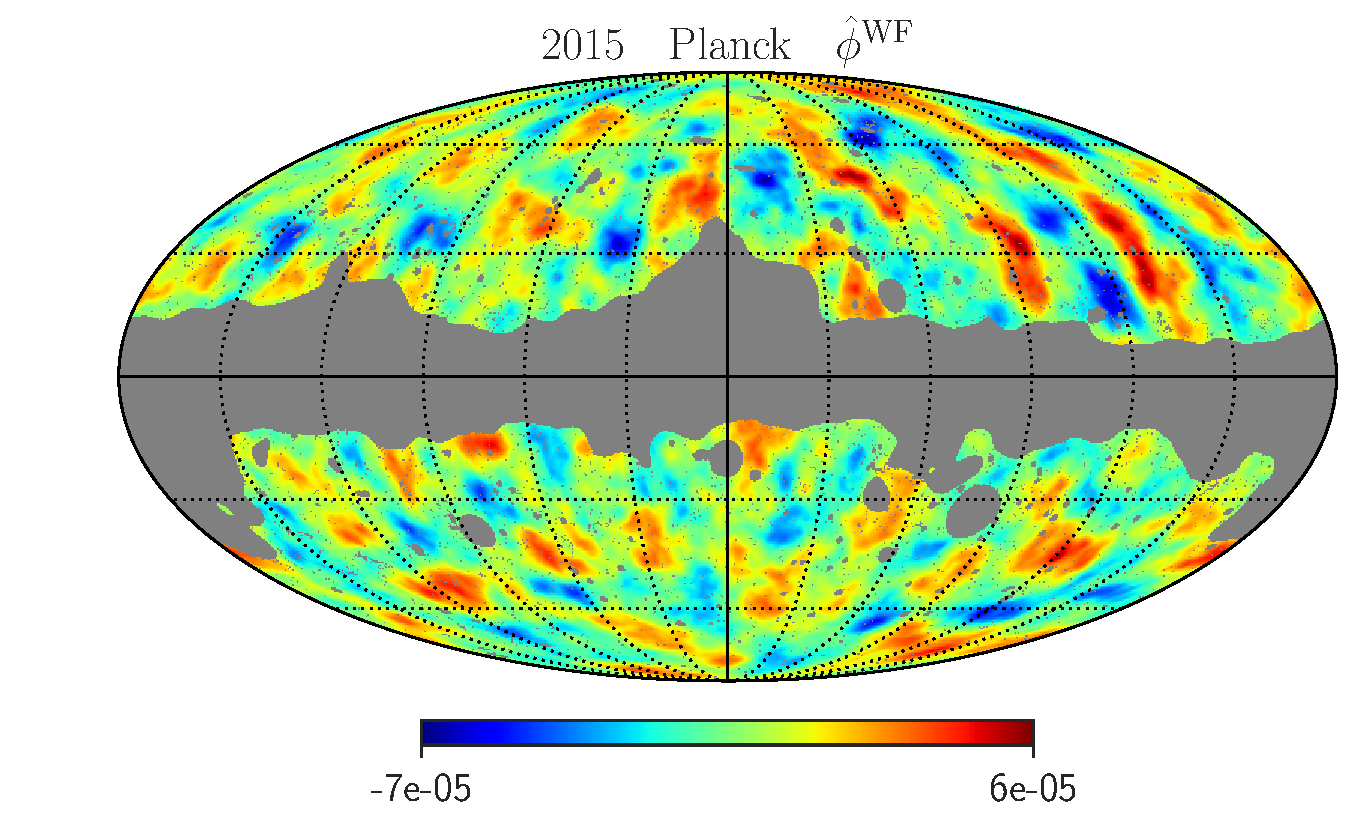
\includegraphics[width=\textwidth]{Chapter2/Images/Planck_kappa_CMB}
\caption{\gls{CMB} lensing potential estimated from \texttt{SMICA} full-mission $T$ and $P$ maps using the MV estimator. The estimate has been Wiener-filtered as $\hat{\phi}^{WF}_{\ell m}= \frac{C_{\ell}^{\phi\phi, \rm{fid}}}{C_{\ell}^{\phi\phi, \rm{fid}}+N_{\ell}^{\phi\phi}}\hat{\phi}_{\ell m}$ for a better visual illustration and the map resolution is $N_{\rm{side}}=512$. \label{fig:planck_kappa}}
\end{figure}


The maps from both data releases are in the \texttt{HEALPix} format with a resolution parameter of $N_{\rm{side}} = 2048$, corresponding to 50331648 pixels over the sky, with a pixel size of $\sim 1.7'$.  In Fig.~\eqref{fig:nlkk_planck} we show the \gls{CMB} lensing reconstruction noise: the flat part at large scales comes from the contribution of the statistical noise, while the rise at smaller scales represents the limitations due to the instrument angular resolution and noise level. As can be seen, the exploitation of the full-mission temperature and the inclusion of polarization data have the effect of augmenting the \emph{Planck} lensing reconstruction sensitivity by approximately a factor of two. Roughly half of the improvement comes from the reduced noise levels in temperature, while the other half comes from the additional polarization data.

\begin{figure}[t] %2
\centering % \begin{center}/\end{center} takes some additional vertical space
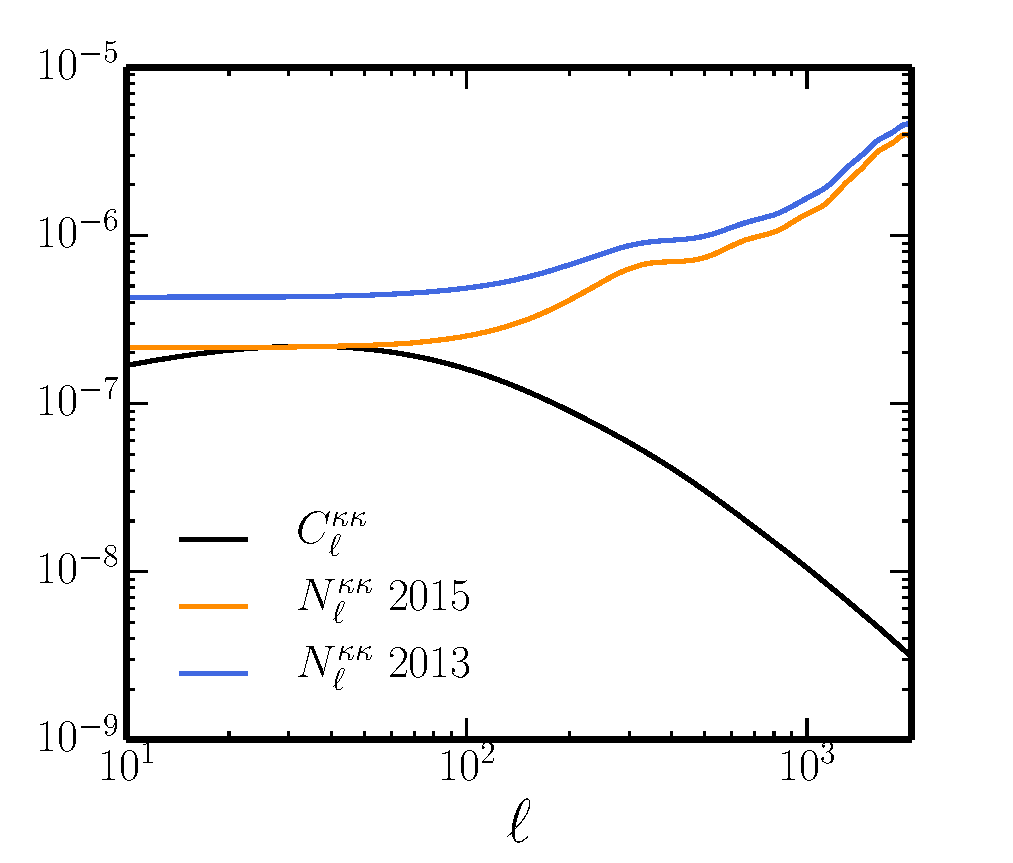
\includegraphics[width=0.5\textwidth]{Chapter2/Images/nlkk_planck_13_15}
\caption{Lens reconstruction noise levels $N_{\ell}^{\kappa\kappa}$ for the 2013 (blue solid line) and 2015 (orange solid line) \textit{Planck} releases. The fiducial \gls{LCDM} \gls{CMB} convergence power spectrum is plotted as the black solid line. \label{fig:nlkk_planck}}
\end{figure}


\subsection{Herschel Space Observatory}
\label{sec:HSO}
The \textit{Herschel} Space Observatory \citep{Pilbratt2010} was launched on the 14th May 2009 together with the \textit{Planck} satellite and represented a huge leap forward in the field of sub-mm/\gls{FIR} astronomy. Before \textit{Herschel}'s arrival, all of the observations were severely limited to small patches, poor angular resolution and a restricted wavelength range was available. However, with its 3.5 m primary mirror\footnote{This is the largest size that could fit within the limits of the Arianne 5 rocket used to ship the satellite into space; in comparison the mirror of \textit{Spitzer}, the next largest \gls{FIR} telescope, is about 0.85m.}, which is the largest one currently in space, \textit{Herschel} has been able to pierce the deep Universe and to observe distant sources. The wavelength coverage of \textit{Herschel} is from 60 to 680 $\mu$m (roughly corresponding to 440 - 5000 Ghz) at diffraction limited resolution, covering most of the dust emission of a typical galactic \gls{SED}. Like \textit{Planck}, the satellite has been placed in the second Lagrangian point to ensure that both the Sun and the Earth were always close to each other, thus limiting contaminations and increasing the available field of view. The detectors on board of \textit{Herschel}, PACS and SPIRE, were able to reach high sensitivities by being cooled down to 0.3 K with liquid ${}^3$He, while most of remaining parts were cooled to 4 - 10 K. The amount of available liquid helium sets the lifetime of the telescope: for \textit{Herschel}, observations have been carried out for approximately 3.5 years. The pointing of the telescope is performed through a combination of gyroscopes and star-tracker cameras: since the launch, the absolute accuracy has been found to be 2'' \citep{Pilbratt2010}.

The telescope carried three main instruments, which are a mixture of broadband photometers and spectrometers: below we provide a brief description.
\begin{itemize}
\item{\textbf{ SPIRE:} The Spectral and Photometric Imaging Receiver (SPIRE) \citep{Griffin2010} consisted of an imaging photometer and medium resolution spectrometer. It carried out observation at $250$, $350$, and $500\,\mu$m band simultaneously (each with a resolution of about $\lambda/\Delta\lambda \sim 3$). The detectors were feedhorn-coupled bolometer arrays with 139, 88, and 43 spider-web bolometers for the three bands respectively. The high sensitivity of SPIRE meant that observations quickly reached the confusion limit, with 1$\sigma$ sensitivities estimated to be around 5.8, 6.3 and 6.8 mJy/beam for the three channels respectively. On the other hand, the SPIRE spectrometer was a medium resolution ($\lambda/\Delta\lambda \sim 1300$ at 200 $\mu$m and $\sim 370$ at $670$ $\mu$m) imaging Fourier transform spectrometer covering 194 - 672 $\mu$m. Science-wise, SPIRE was able to shed light on the sub-mm region least explored by previous instruments, thus allowing an investigation of the cold and dusty Universe.}

\item{\textbf{ PACS}: The Photodetector Array Camera and Spectrometer (PACS) \citep{Poglitsch2010} was a photometer and medium resolution spectrometer operating in the 60 - 210 $\mu$m regime. The photometer performed observations in three bands centered in 70, 100, 160 $\mu$m (with $\lambda/\Delta\lambda \sim 2$) and could observe either the 70 or 100 $\mu$m channel simultaneously with the 160 $\mu$m band. The mounted spectrometer was a medium resolution spectrometer ($\lambda/\Delta\lambda \sim 1000 - 4000$) covering the wavelengths range between 55 and 210 $\mu$m. PACS provided photometric observations of the peak of galactic dust emission in the nearby Universe at high spatial resolution; its main  scientific goals  were to map the spectral lines in the \gls{FIR}, in the Milky Way and in local galaxies.}

\item{\textbf{ HIFI}: The \textit{Herschel}-Heterodyne Instrument for the Far-Infrared (HIFI) was the high resolution spectrometer operating in the broad wavelengths range between 157 and 625 $\mu$m. Unlike SPIRE and PACS, it only had a single pixel but maps could be made using either a series of pointing or on-the-fly mapping. The main scientific target of the instrument was to investigate the interaction between stars and the interstellar medium in galaxies by searching for molecular rotational lines.}
\end{itemize}

Several surveys have been carried out with the \textit{Herschel} telescope. In this thesis we have made use of data gathered in the context of the H-ATLAS \citep{Eales2010a}, here we give a brief overview.

The H-ATLAS is the largest extragalactic key-project carried out in open time with the \textit{Herschel} Space Observatory. It was allocated 600 hours of observing time and covers about $600\,\hbox{deg}^2$ of sky in five photometric bands (100, 160, 250, 350 and $500\,\mu$m) with the PACS and SPIRE instruments. The H-ATLAS map-making is described by \citet{Pascale2011} for SPIRE and by \citet{Ibar2010} for PACS. The procedures for source extraction and catalogue generation can be found in \citet{Rigby2011} and \citet{Valiante2016}. 

Since H-ATLAS is an extragalactic survey, the observed fields were chosen to minimize the Galactic dust contamination. As such, the survey area is divided into five fields: three equatorial fields centered on 9hr, 12hr, and 14.5hr (Galaxy And Mass Assembly (GAMA) fields, G09, G12, and G15) covering, altogether, $161\,\hbox{deg}^2$; the North Galactic Pole (NGP) block, a rectangular block of $15^\circ\,\cos(\delta)$ by $10^\circ$ centered on right ascension $\alpha=199.5^\circ$, declination $\delta=29^\circ$ and rotated by approximately $8^\circ$ clockwise; and the South Galactic Pole (SGP) block consisting of two concatenated rectangular regions, one of $31.5^\circ\cos(\delta)$ by $6^\circ$ centered on $\alpha=351.3^\circ$, $\delta=-32.8^\circ$, the other of $20^\circ\cos(\delta)$ by $6^\circ$ centered on $\alpha=18.1^\circ$, $\delta=-30.7^\circ$. The fields were also chosen depending on the amount of complementarity data available from external surveys operating at different frequencies. For example, spectroscopy is covered by GAMA, Sloan Digital Sky Survey (SDSS), and 2dF Galaxy Redshift Survey (2dFRGS), while much of the area has been covered by Galaxy Evolution Explorer (GALEX) in the ultraviolet.  As concerns optical wavelengths, the SDSS has covered both the GAMA and NGP fields in five bands, while GAMA and SGP fields have been observed by the Kilo Degree Survey (KIDS); the SGP will be eventually covered by the Dark Energy Survey (DES).

The scientific targets of H-ATLAS are multiple, concerning both the local and the distant Universe. In particular, a huge number of the discovered objects do not belong to the local Universe: \textit{Herschel} is able to resolve the \gls{CIB} into discrete sources, thus enabling an investigation of the \gls{LSS} of the \gls{FIR} Universe.
The $z\lesssim 1$ galaxies detected by the H-ATLAS survey are mostly late-type and starburst galaxies with moderate star-formation rates and relatively weak clustering  \citep{Dunne2011,Guo2011}. High-$z$ galaxies are forming stars at high rates ($\ge \hbox{few hundred}\,\hbox{M}_\odot\,\hbox{yr}^{-1}$) and are much more strongly clustered \citep{Maddox2010,Xia2012}, implying that they are tracers of large-scale overdensities. Their properties are consistent with them being the progenitors of local massive elliptical galaxies \citep{Lapi2011}. These \gls{DSFG} contain a substantial amount of dust and as a consequence, their rest-frame optical/ultraviolet (UV) light can be strongly obscured. It is this high-$z$ H-ATLAS galaxy population that we aim to correlate with the \textit{Planck} CMB lensing map in Ch.~\eqref{ch:xc1} and~\eqref{ch:xc2}. In order to select the these galaxies into a catalogue and, as an example, slice them in bins for a tomographical analysis, the knowledge of their redshift must be at hand. Unfortunately, redshift acquisition is not straightforward for dusty \gls{IR} selected objects: this is because most of the emission-line redshift indicators lie in the rest-frame optical and UV bands that are severely extinct by dust, and because \gls{IR} observations are carried out with large beam sizes that make multiband counterpart identification ambiguous. A common method to determine the millimetric photo-$z$, is to perform a \gls{SED} fitting in the \gls{FIR}, where redshifts are estimated from the shape of the \gls{FIR}/sub-mm \gls{SED} or its colors rather than properties indicated by its stellar emission features in the optical or emission-lines signatures. Differently from data in the optical or near-\gls{IR}, \gls{FIR} data lacks of an extensive photometric wavelength coverage: at most, individual galaxies will have around 10 photometric points in the \gls{FIR} (and an average of 3-5), while in the optical it is common to have more than 30 bands \citep{Casey2014}. The basic idea assume that the far-\gls{IR} \gls{SED} is roughly fixed (e.g. to SMM-J2135 or Arp220) and then to use the \gls{FIR} colors to infer the galaxy's redshift\footnote{Of course the accuracy of the method is dependent on the intrinsic variation in \gls{SED} types within a given population and as a consequence the precision can be poor.}, allowing for a study of the redshift distribution in a statistical sense rather than for individual galaxies. \gls{SED} fitting process can be divided into (i) methods that compare directly data (i.e. fluxes or colors) with model templates by means of $\chi^2$ or Bayesian techniques, and (ii) methods that fit for simple modified greybody-like functions. The baseline method used here to infer galaxies photo-$z$ is the former and will be discussed in Ch.~\eqref{ch:xc1} and~\eqref{ch:xc2}. The main feature of the \gls{FIR} \gls{SED} is the presence of a peak due to dust emission (see Fig.~\eqref{fig:SED_SMM}); however, note that the dust temperature (which manifests as the \gls{SED} peak wavelength) correlates with \gls{IR} luminosity and can be degenerate with redshift. The radial distribution of H-ATLAS galaxies is shown in Fig.~\eqref{fig:hatlas3D}.


\begin{figure} %3
\centering % \begin{center}/\end{center} takes some additional vertical space
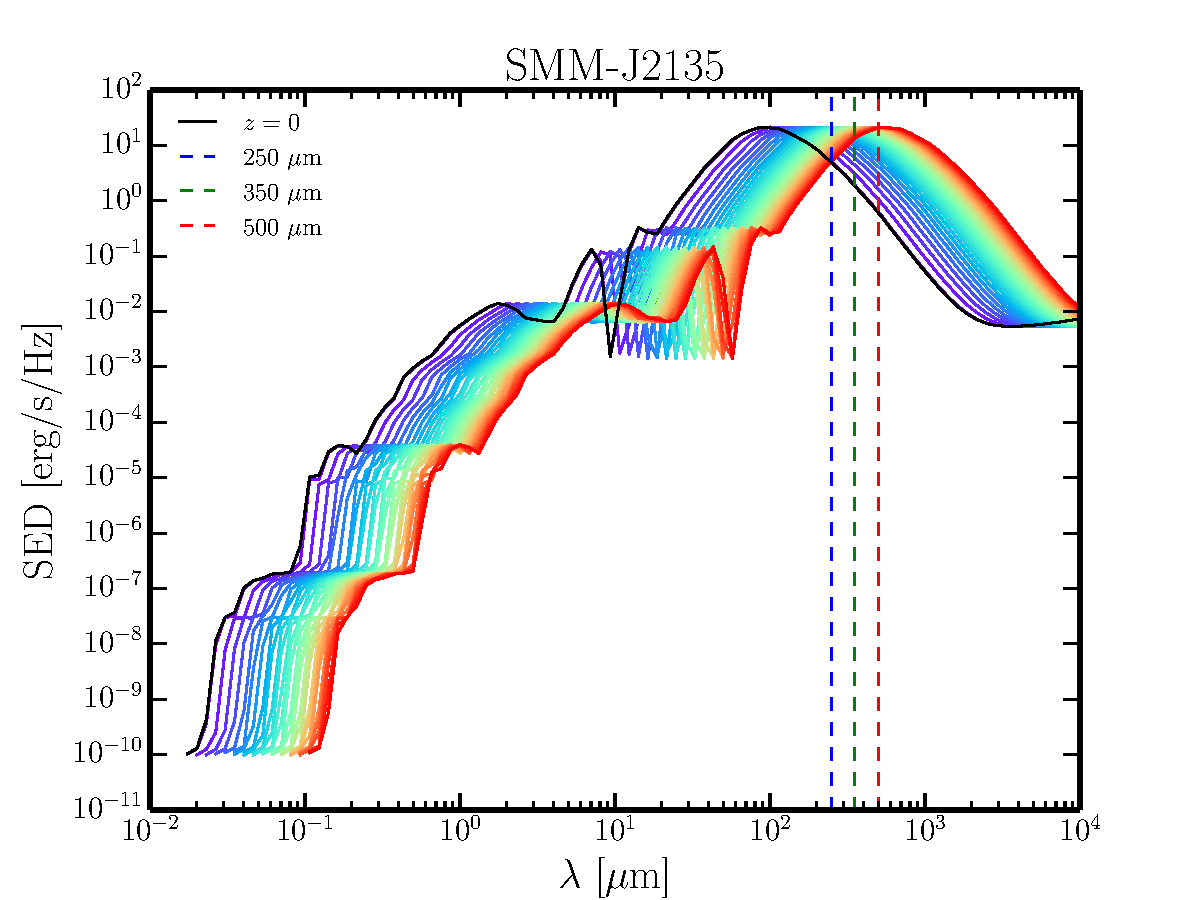
\includegraphics[width=0.8\textwidth]{Chapter2/Images/SED_zs}
\caption{SMM SED template  at $z=0$ (black solid line): solid colored lines from purpleish to reddish represent rest-frame SED \emph{redshifted} in the range $0 < z \le 5$. Colored dashed lines mark the wavelengths observed by the SPIRE photometer instrument on board of the Herschel satellite. The prominent \emph{moving} peak that enables the photo-$z$ determination with three photometric points is clearly visible.  \label{fig:SED_SMM}}
\end{figure}




\begin{figure} %3
\centering % \begin{center}/\end{center} takes some additional vertical space
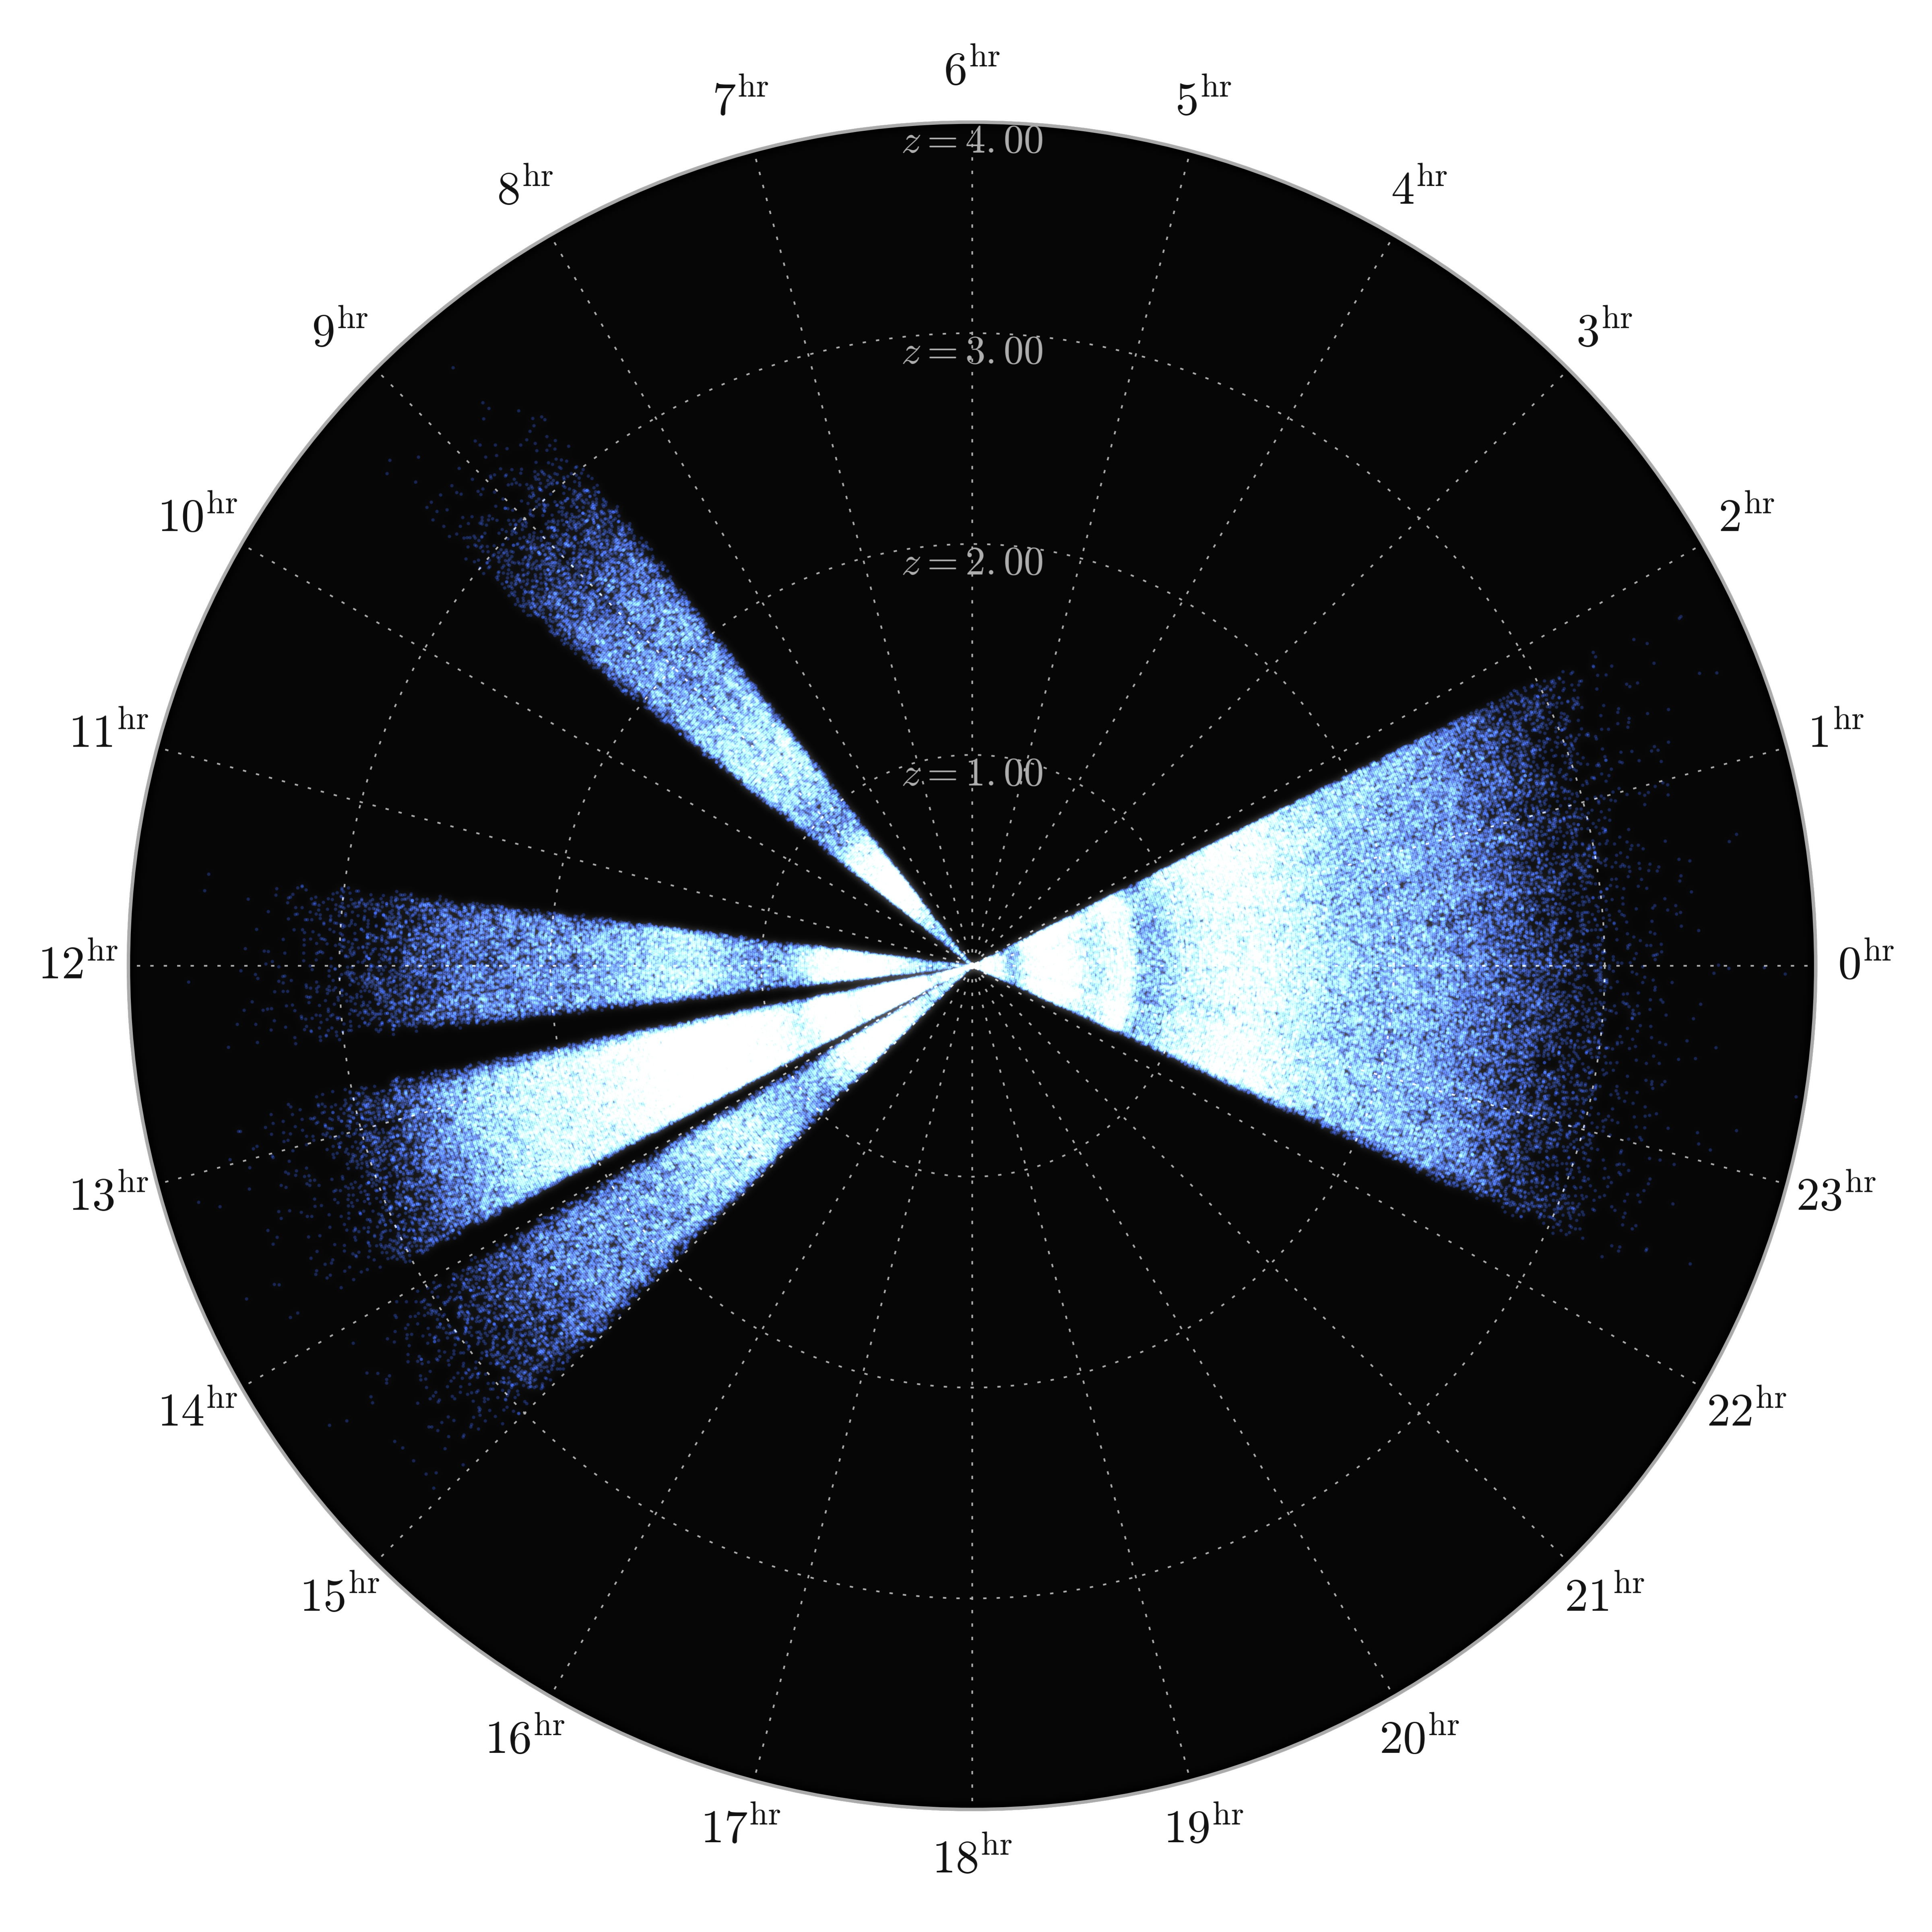
\includegraphics[width=\textwidth]{Chapter2/Images/hatlas3d}
\caption{Angular and radial distribution of sub-mm galaxies in all of the five H-ATLAS patches. 
Please note that \textit{photometric} redshifts have been used to place galaxies along the redshift
axis and even though the spongy structure of the matter distribution is hardly observed - given the photo-$z$ 
uncertainties that can be important - the radial information can be used in a statistical way. 
In fact, the two main populations at $z \lesssim 1$ and at $z \gtrsim 1$ can be seen. \label{fig:hatlas3D}}
\end{figure}
